\documentclass[10pt, a4paper]{article}

\usepackage{geometry}
 \geometry{
 a4paper,
 total={210mm,297mm},
 left=25mm,
 right=25mm,
 top=30mm,
 bottom=25mm,
 headsep=7mm}

\usepackage{graphicx}
\usepackage{todonotes}
\usepackage{hyperref}
\usepackage{listings}
\usepackage{enumerate}
\usepackage{fancyhdr}
\usepackage{longtable}
\usepackage{comment}
\usepackage{lipsum}
\usepackage{multicol}
\usepackage{wrapfig}


\graphicspath{ {images/} }

\pagestyle{fancy}
\fancyhf{}
\fancyhead[L]{\leftmark}
\fancyfoot[C]{\thepage}
\renewcommand{\headrulewidth}{0.4pt}

\begin{document}

	\begin{titlepage}
		\centering
		% logo image
		
\includegraphics[scale =0.8]{logo.jpg}\par\vspace{1cm}
		% institution 
		{\scshape\LARGE\bfseries Ecole Polytechnique de Louvain\par}
		\vspace{1.5cm}
		{\scshape\Large \par}
		\vspace{1.5cm}
		% title
		{\huge\bfseries LINGI2364: Mining Patterns in Data \par}
		\vspace{1cm}
		{\Huge Project 2: SequenceMining \par}
		\vspace{2cm}
		{\LARGE Group 11\par}
		% versioning
		\vspace{1cm}
		% author
		{\Large\itshape Alessandra Rossaro (01211800), Matteo Salvadore (01731800)\par}
		\vspace{2cm}
		{\small Version 1.0 - 18/11/2018\par}

		\vfill

		% Bottom of the page
		{\large AY 2018-2019\par}
	\end{titlepage}

	\section{Implementations}
	The implementations of our algorithms are performed in Java language (JDK 8 ).
	The source code and all the resources used to perform this project are available in the following GitHub repository: \url{https://github.com/JustSalva/ProjectsOfMiningPatternsInData}.\newline\newline
	We have chosen to structure our algorithms in a hierarchical way: the backbone of our entire second assignment is an implementation of the \textit{PrefixSpan} algorithm, performed in an abstract class (\textit{GenericAlgorithm}) that contains all the necessary structures to perform the depth-first search, but leaves details like the evaluation functions, pruning constraints, and all methods that handle the k-best pattern management (threshold update when a better score is found, initial management of the list containing the best k patterns and heuristic function for the node's expansion) to the subclasses that extend our abstract class (one for each task of the assignment).
	The transactions are read from the data-sets and stored in a custom structure we have built; the structure consists in a unique hash-map (in order to perform direct accesses =$>$ O(1) complexity), we have used a boolean flag to distinguish the transactions belonging either to the positive data-set and to the negative one.\newline
	\begin{wrapfigure}[]{h}{0.5\textwidth}
		\centering
		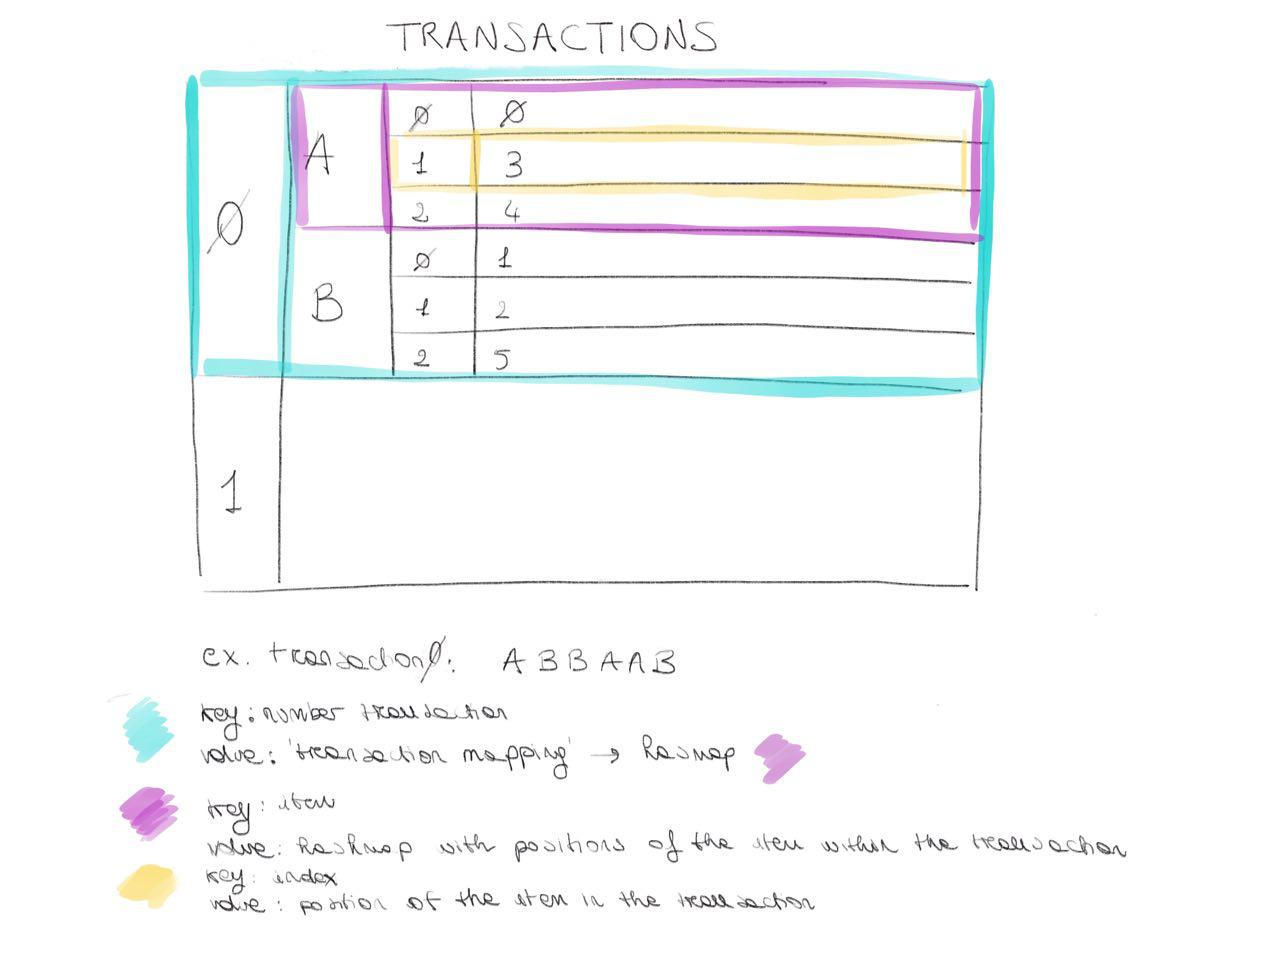
\includegraphics[scale =0.25]{transactions.jpg}
		\caption{{\small  transactions: graphical representation}}
		\vspace{0.5cm}
		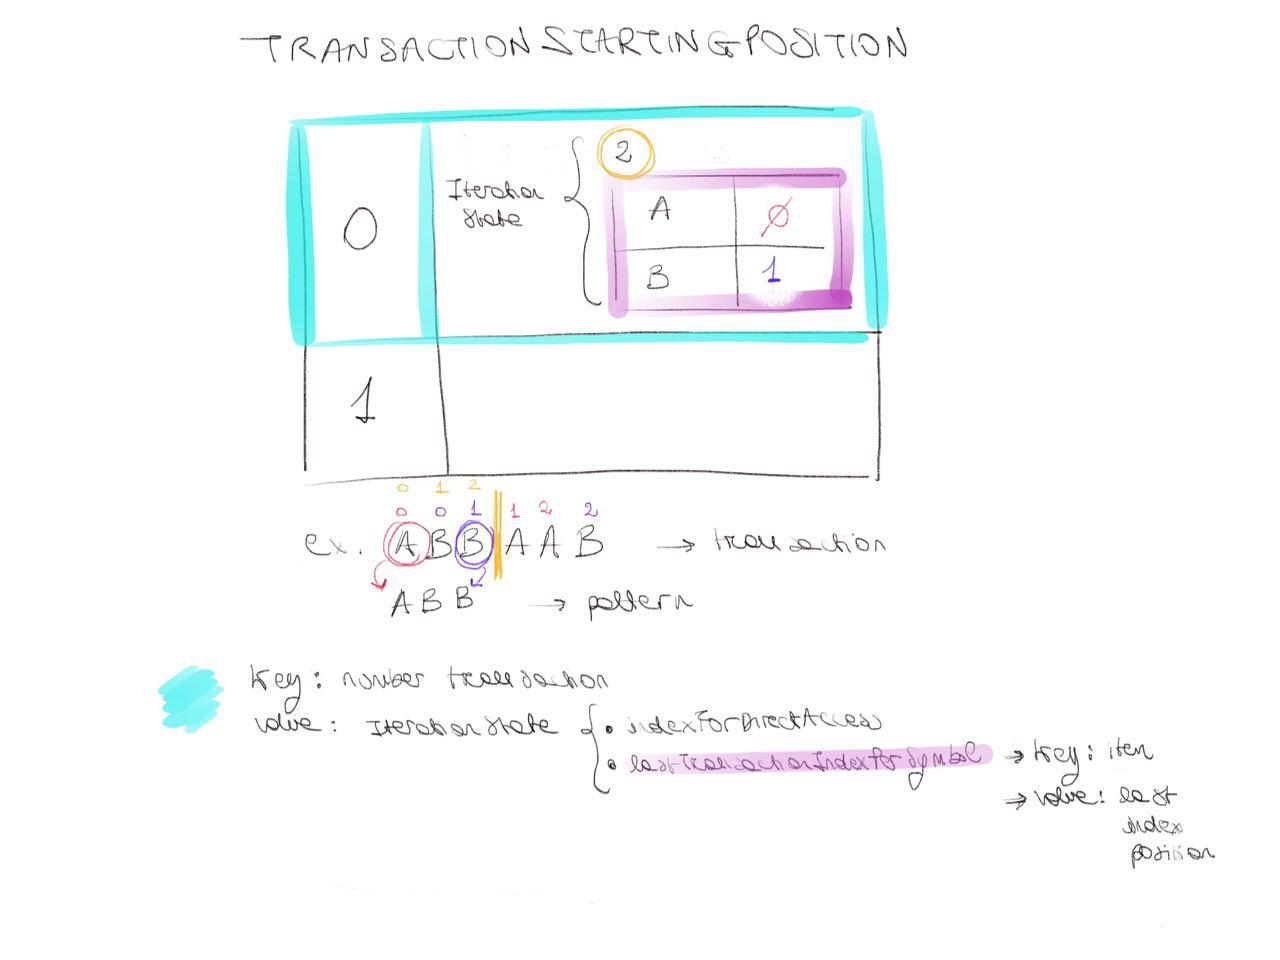
\includegraphics[scale =0.25]{transactionStartingPosition.jpg}
		\caption{{\small transactionStartingPosition: graphical representation}}
	\end{wrapfigure}
	We have chosen to not build a proper projected data-set (coping each time the transactions), but we have decided to create an optimized structure that is faster to access and lighter in memory. It consists in a hash-map that contains as key the transaction number and as value another hash-map that contains as key the singular item (e.g. A,B,...) and as value another hash-map that contains as key an incremental index and as value the positions of the item in the transaction. We give you a graphical representation of our structure on the right [Figure 1].
	\newline
	Our projected database saves only the positions of the items within the transaction so we do not need to copy the entire data-set, but we just copy the last visited index of each item in each transaction. 
	The structure of this projected database is an hash-map that contains as key the number of transaction (only the transactions that contain the pattern belonging to the tree's node) and as value an object called \textit{IterationState} that contains:
	\begin{itemize}
		\item An index, used to perform direct access, (\textit{indexForDirectAccess}) that corresponds to the last position of the element read from the transaction.
		\item An hash-map that contains as key the singular item (e.g A,B,...) and as value an index that corresponds to the last incremental index of each singular item (see the previous structure) that represents the last value of that symbol used to form the pattern for which the database is projected.
	\end{itemize}
	We give you a graphical representation of our structure on the right [Figure 2].\newline
	\noindent
	We have decided to expand nodes using an heuristic function that uses the item's score (to be defined in the subclasses). The nodes that have to be expanded are stored in a priority queue, ordered by descending item's score value. In this way the probability to find the best patterns is improved, but the expansion of nodes is no more in depth.\newline
	When we have to expand a node we consider only the singular items that were still frequent during the exploration of the father node, in this way we avoid useless searches of items for which we know that cannot be present in the pattern anymore.
	\newline\newline
	Since during the expansion of nodes the threshold is not known a priori, but can be continuously updated during the search, we have to perform some kind of filtering before returning the found patterns and so we do this by inserting them in a list containing the found patterns in reverse order of score (N.B. to be implemented by each subclass) and delete the ones that are no more part of the k-best patterns.

	\subsection{Frequent sequence mining}
	In this task we have provided the \textit{PrefixSpan algorithm} with a TreeSet called \textit{maxValuesOfK} that keeps the K best support values (Integers) and when the algorithm computes better values it updates the Set. The threshold that we have applied in order to prune the search is the minimum value of this Set.\newline
	In order to check the constraints we have implemented a method called \textit{checkConstraints} that evaluates the threshold and, if necessary, it updates the Set and the minimum value. Obviously the evaluation function,for this implementation, computes the sum of the supports of both positive and negative data-sets.
	We can prune the search with the described rule since the support is anti-monotonic.

	\subsection{Supervised sequence mining}
	In this task the management of the K best Wracc values is handled in the same way of the previous task, the only difference is that in this case the values are floats instead of integers, since the evaluation function (\textit{Wracc}) has as domain the Real numbers' set.
	Since the \textit{Wracc} is not anti-monotonic we cannot prune the search if we obtain a lower value respect of minimum value, so we have applied a lower bound computed with the formula $p\geq minWracc*\frac{(N+P)^2}{N}$ obtained putting the \textit{n} (number of negative examples) equal to zero in the \textit{Wracc} inequality constraint ($Wracc \geq threshold$).
	
	\subsection{Supervised closed sequence mining}
	In this task we have simply extended the \textit{Supervised sequence mining} class, since the algorithm is the same and we just had to filter the final results in order to keep only the closed patterns.
	This filtering process is computed in our \textit{printResults} function. In order to perform only the minimal number of comparisons we have ordered the candidate patterns (with the same support) from the shortest to the longest one and then we have compared them, checking if the shortest one was a substring of the longer patterns: if it was not contained, it was saved in the list of the results and in both cases, after the comparison, the first element was removed from the list.	
		
	\subsection{Alternative scoring functions}	
	\subsubsection{Absolute value of Wracc score}	
	For this task we have extended the \textit{Supervised closed sequence mining} class. The only changes are:
	\begin{itemize}
		\item The evaluation function uses the absolute value of the \textit{Wracc} function; doing so we have included also the patterns that are strongly present in the negative class.
		\item Since the evaluation function has changed we have added another constraint that is the symmetrical formula w.r.t. the constrain explained in Section 1.2 (N.B. due to the absolute value): \newline $n\geq minWracc*\frac{(N+P)^2}{P}$.
	\end{itemize}

	\subsubsection{Information Gain}
	For this task we have extended the \textit{"Absolute value of Wracc score"}'s class. The only changes are:
	\begin{itemize}
		\item The evaluation function uses the \textit{Information Gain} formula.
		\item Since the evaluation function has changed we have changed constraints, that are implemented in the following way: given a pattern's pair \textit{(n,p)} where \textit{p} is the number of positive examples and \textit{n} the number of negatives ones, we have computed the \textit{Information Gain} score for the pairs \textit{(0,p)} and \textit{(n,0)}. These two values were compared with the minimum information gain score (minimum in the k best patterns), if both values were lower than the minimum we pruned the search.	
	\end{itemize}
	\section{Analysis of patterns found}
	We have decided to insert in the report the analysis with a value of k equal to 6 and with the test data-set, however the same observations can be performed with all the other examples (for more info see\textit{ src/main/resources/Performances} folder in our repo's second assignment folder).
	\begin{center}
	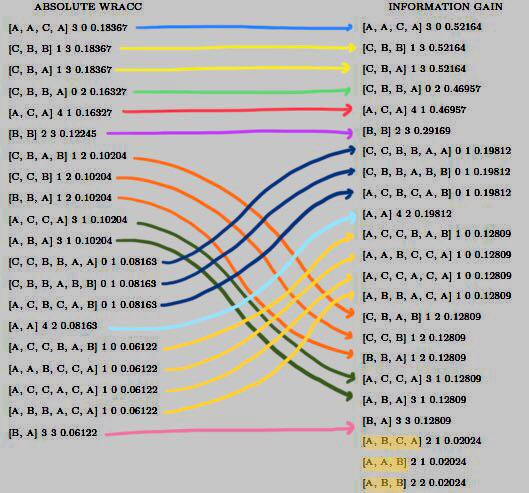
\includegraphics[scale =0.8]{patterns.jpg}\par\vspace{1cm}
	\end{center}
	\noindent
	Looking at the picture we can notice that the evaluation function that uses the \textit{Information Gain} obtains more values than the evaluation function that uses the \textit{Absolute Wracc}. This could be caused because the first function uses an approach more probabilistic and based on entropy and so it could consider a wider set of solutions.
	However, the majority of patterns are in common for both functions and so we cannot appreciate strong differences; obviously the values of the evaluation functions are different for the same patterns, but looking at their relative order we notice that the \textit{Information gain} formulation advantages longer patterns w.r.t. shorter ones
	\section{Performances}
	In this section we discuss about the performance in terms of time, expressed in milliseconds, for the three provided datasets: \textit{Tests}, \textit{Proteins}, \textit{Reuters}. 
	We have decided to present them in three different graphics because the orders of results are very different for each data-set and didn't allow to properly visualize the behavior of the five algorithms applied to the different data-sets.
	As expected the execution time grows as the values of k grows, since the algorithms can apply stricter pruning rules with smaller values of k.\newline
	We notice that the \textit{Information Gain} algorithm suffers more for the higher branching factor of the \textit{Reuters} dataset, but overall the Wracc (and closed Wracc) algorithm are the most computationally expensive, while the prefix span is the least expensive one.

	\begin{multicols}{2}
	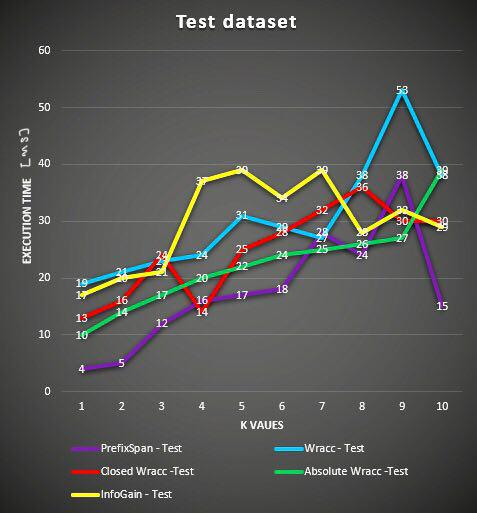
\includegraphics[scale=0.5]{tests.jpg}
	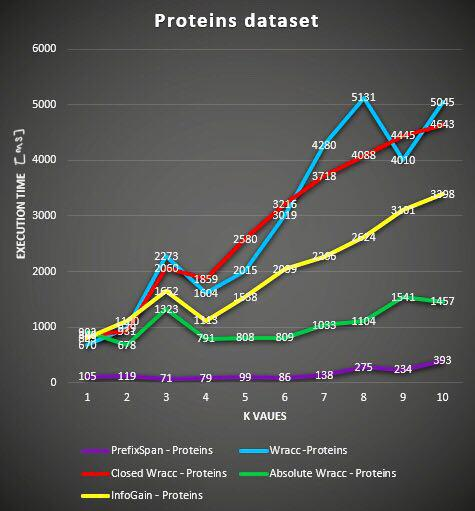
\includegraphics[scale=0.5]{proteins.jpg}	
    \end{multicols}
	\begin{center}
	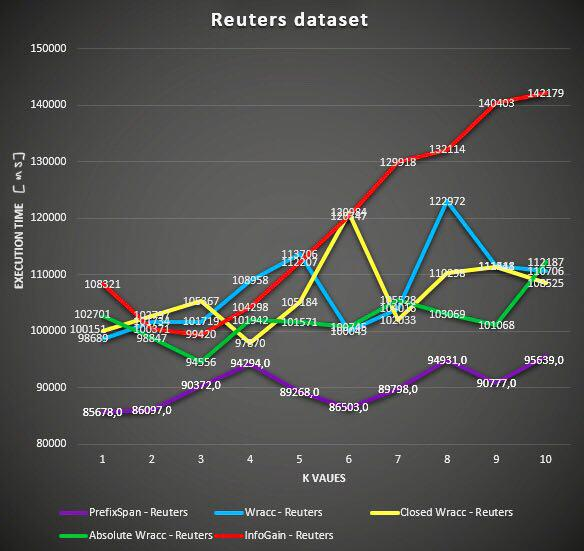
\includegraphics[scale =0.45]{reuters.jpg}
	\end{center}

	\section{Our system specification}
		All our measurements have been tested on a laptop with the following specifications:
		\begin{multicols}{2}
			\begin{itemize}
				\item Processor: Intel® Core™ i5-6198DU CPU @ 2.30GHz x 4 
				\item RAM: 12 GiB - DDR4
				\item OS: Ubuntu 18.04.1 LTS
				\item JRE: Java 8u191
			\end{itemize}
		\end{multicols}
	
	\section{Notes}
	The biggest difficulties that we have encountered were linked to the development of the backbone structure of our system, because our idea was to create a general enough structure that could support all the required implementations. Once built, we have not encountered big problems to implement the required algorithms. Another difficulty that we have encountered was the optimization of the code in order to analyze the Reuters data-set, that was way bigger than the other data-sets and its tree-search's branching factor was huge. Nonetheless once reached a good level of optimization (due to our optimized data structures), the hierarchical nature of our implementations  this had been crucial to exploit those optimizations for all algorithms.
		

\end{document}
